% Insertar en Evaluación Estadística y Eficiencia, sin reemplazar Cacho.
% 13. Métodos Estadísticos Requeridos; 13.1. Ejemplo de Análisis Requerido; 14. Evidencia Formal de Eficiencia.
\subsection{Othello: metodología estadística y eficiencia}
\textit{Guía: 12.1. Para Othello, punto 2; 13. Métodos Estadísticos Requeridos; 14. Evidencia Formal de Eficiencia.}
La apertura es la unidad de remuestreo; se conservan juntas las partidas de ambos colores y se separan las profundidades. Se define victoria de bloque si A obtiene más de un punto en sus dos partidas. El test binomial exacto bilateral contrasta $H_0:P(\text{A gana bloque}\mid\text{bloque decisivo})=0.5$; excluye bloques empatados y aplica Holm entre comparaciones. No es el mismo estimando que la victoria por partida. Los intervalos Wilson al 95\% sobre partidas se rotulan descriptivos por su dependencia; se añade Wilson por bloque decisivo \cite{wilson1927interval,othello_nist_wilson}.

El bootstrap percentil remuestrea medias por apertura (5000 réplicas, semilla 20261008) para diferencia de fichas y proporción de victorias \cite{othello_efron1979}. Con sólo un bloque por profundidad no se estima un intervalo bootstrap informativo. Chi-cuadrado no se aplica al round-robin emparejado: las filas de rivales comparten partidas; el código lo reserva para muestras independientes y frecuencias esperadas al menos 5 \cite{othello_nist_chi}. El ejemplo unilateral 58/100 de 13.1. Ejemplo de Análisis Requerido no debe confundirse con nuestro contraste bilateral.

Para Pearson/Spearman se fijan profundidad, función y colocación (20,30,40,50). Se relacionan evaluaciones medias por apertura desde negras con la diferencia final media negras menos blancas. No se mezclan perspectivas ni se tratan varias posiciones de una partida como independientes. El piloto tiene un bloque: las correlaciones entre bloques no son estimables. La herramienta permite obtenerlas, junto con permutación bilateral e intervalos bootstrap, cuando existan suficientes aperturas; serán exploratorias y no causales.

Evaluar una posición cuesta $O(n^3)$; explorar el árbol tiene peor caso $O(b^d n^3)$, omitiendo aquí el ordenamiento $O(b\log b)$ por nodo. Las mediciones log-log no demuestran crecimiento polinomial en $d$. El punto 3 de 14. Evidencia Formal de Eficiencia contiene esa exigencia incompatible con la cota general; se explicita y queda pendiente aclararla con el docente. Las trayectorias de partida cambian con $d$, por lo que se proporciona además un benchmark sobre matrices fijas.
% 14. Evidencia Formal de Eficiencia, punto 3. Generado por analizar.py.
Se registraron 16 decisiones sobre posiciones fijas, separadas de las partidas del torneo. 
En la posición inicial, 
a profundidad 4 se midieron entre 0.0237 y 0.0242 segundos; 
a profundidad 7 se midieron entre 1.4145 y 1.4857 segundos; 
estos extremos corresponden a las condiciones medidas, no a un intervalo de confianza. 
En la posición tras 50 colocaciones, 
a profundidad 4 se midieron entre 0.0174 y 0.0251 segundos; 
a profundidad 7 se midieron entre 0.3437 y 0.3613 segundos; 
estos extremos corresponden a las condiciones medidas, no a un intervalo de confianza. 
Se conserva una medición por condición en este piloto; no se estima variabilidad ni se demuestra crecimiento polinomial.

\begin{figure}[htbp]
\centering
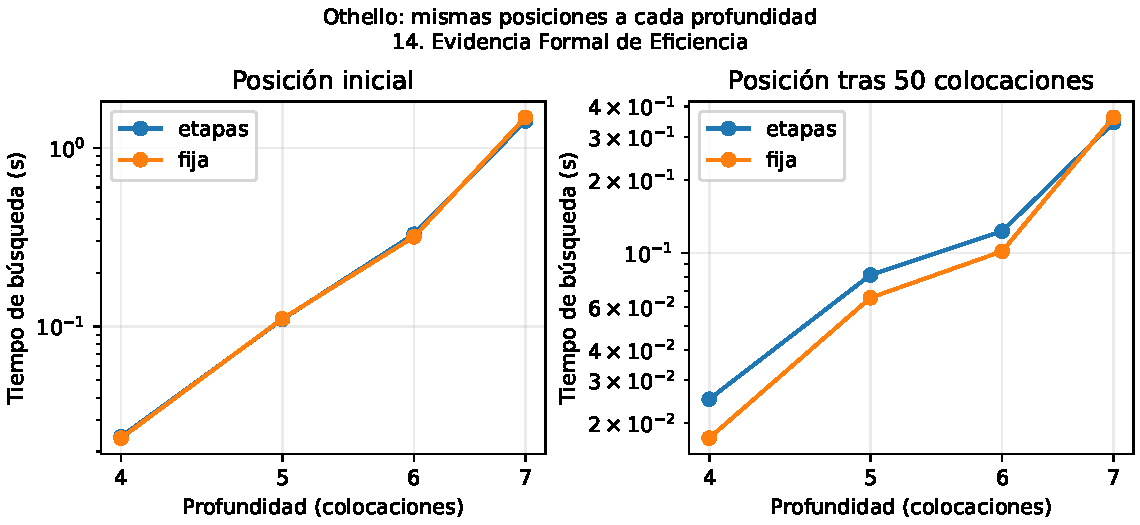
\includegraphics[width=.95\linewidth]{../datos/othello/analisis/benchmark_loglog_othello.pdf}
\caption{Tiempo de búsqueda en escala log-log sobre dos matrices fijas, conservando el turno real. Una medición por versión, posición y profundidad; sin ajuste ni afirmación de ley polinomial.}
\label{fig:othello_loglog}
\end{figure}
